\section{Reinforcement Learning \points{24}} 

Consider an environment in which our agent requires caffeine to function (if it helps, you can think of the agent as a graduate student). Because caffeine is so important to our agent, we would like the agent to find a policy that will always take the shortest path to coffee. \\

In order to apply reinforcement learning techniques such as value iteration and policy iteration, we first need to model this scenario as a Markov decision process (MDP). Note that there may be many different ways to define each of the MDP components for a given problem. Recall that an MDP is defined as a tuple
$(S, A, P, R, \gamma)$ where:
\begin{itemize}
\item[$S$] is the (finite) set of all possible states.
\item[$A$] is the (finite) set of all possible actions.
\item[$P$] is the transition function $P: S \times S \times A \to [0, 1]$, 
  which maps $(s', s, a)$ to $P(s'|s, a)$, i.e., 
  the probability of transitioning to state $s'\in S$ when taking action
  $a\in A$ in state $s\in S$. 
  Note that $\sum _{s' \in S} P(s' | s, a) = 1$ for all 
  $s \in S, a \in A$.
\item[$R$] is the reward function $R : S \times A \times S \to \mathbb R$,
which maps $(s, a, s')$ to the real-valued reward $R(s, a, s')$, i.e., 
the reward obtained when taking action $a \in A$ in state $s \in S$ and 
arriving at state $s' \in S$.
\item[$\gamma$] is the discount factor, which controls the relative importance of short-term and long-term rewards. We generally have $\gamma \in [0, 1)$ (i.e., $0 \leq \gamma < 1$), where smaller values mean greater  discounting of future rewards.
\end{itemize}

For this problem, we represent the state of the agent at any time by the triple $(x, y, o)$, where $x$ and $y$ are the horizontal and vertical coordinates of the agent's location, respectively, and $o$ is the agent's orientation which is one of $\{ N, E, W, S \}$ (North, East, West, South). The agent's current orientation is the only direction it can move. The agent is able to move forward, turn right, or turn left (deterministically). All actions are available in all states. More specifically, the action space is $|A| = \{F,R,L\}$ where:
\begin{itemize}
\item F (move Forward): The agent moves forward one cell along its current orientation, changing the agent's location but not its orientation.
\item R (turn Right): The agent turns right, changing the agent's orientation but not its location.
\item L (turn Left): The agent turns left, changing the agent's orientation but not its location.
\end{itemize}
Walls are represented by thick black lines. The agent cannot move through walls. If the agent attempts to move through a wall,  it will remain in the same state.

When the agent reaches the coffee cup in any orientation, the episode ends. Another way to think of this is that every action in the coffee cup state keeps the agent in the coffee cup state.


\begin{figure}[h]
  \centering
  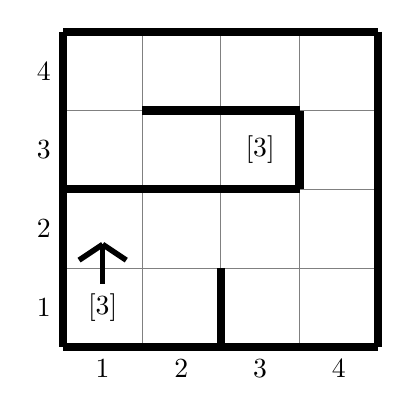
\begin{tikzpicture}
    \draw[step=1cm,gray,very thin] (0,0) grid (4,4);
    \foreach \x in {1, ..., 4}
      \draw (\x cm - .5cm, 1pt) -- (\x cm - .5cm, -1pt)
      node[anchor=north] {$\x$};
      \foreach \y in {1, ..., 4}
      \draw (1pt,\y cm - .5cm) -- (-1pt, \y cm - .5cm)
      node[anchor=east] {$\y$};

      % Agent
      \node (agent) at (.5cm, .5cm) { \Strichmaxerl[3]};
      \draw[line width=2pt] (0.5cm, 0.8cm) -- (0.5cm, 1.3cm);
      \draw[line width=2pt] (0.5cm, 1.3cm) -- (0.2cm, 1.1cm);
      \draw[line width=2pt] (0.5cm, 1.3cm) -- (0.8cm, 1.1cm);
      
      % Goal
      \node (goal) at (2.5cm, 2.5cm) {\Coffeecup[3]};

      % Obstacles
      \draw[line width=3pt] (2cm, 0cm) -- (2cm, 1cm);
      \draw[line width=3pt] (0cm, 2cm) -- (3cm, 2cm);
      \draw[line width=3pt] (3cm, 2cm) -- (3cm, 3cm);
      \draw[line width=3pt] (3cm, 3cm) -- (1cm, 3cm);
      \draw[line width=3pt] (4cm, 4cm) -- (4cm, 3cm);

      % Border
      \draw[line width=3pt] (0cm, 0cm) -- (0cm, 4cm);
      \draw[line width=3pt] (0cm, 0cm) -- (4cm, 0cm);
      \draw[line width=3pt] (4cm, 4cm) -- (0cm, 4cm);
      \draw[line width=3pt] (4cm, 4cm) -- (4cm, 0cm);
  \end{tikzpicture}
  \caption{\label{fig:prob1_shortest_path_domain} MDP for Problem 1, Part I. The goal is for the agent to have a policy that always leads it on the shortest path to the coffee at coordinate $(3,3)$. In this instance, the agent's current state is $(1,1, N)$ }
\end{figure}
\newpage
Consider the instance shown in Figure~\ref{fig:prob1_shortest_path_domain}. The goal, displayed as a coffee cup, is located at $(3,3)$. Using the above problem description answer the following questions:

\begin{enumerate}
\item {[\textbf{1 point}]} i.) How many states are in this MDP? 
\begin{tcolorbox}[fit,height=1cm, width=2cm, blank, borderline={1pt}{-2pt}]
        %solution 
\end{tcolorbox}


[\textbf{1 point}] ii.) How many actions are in this MDP?
\begin{tcolorbox}[fit,height=1cm, width=2cm, blank, borderline={1pt}{-2pt}]
            %solution 
        \end{tcolorbox}


 [\textbf{1 point}] iii.) What is the total number of  entries in the transition table of $T(s'\mid s, a)$?
\begin{tcolorbox}[fit,height=1cm, width=4cm, blank, borderline={1pt}{-2pt}]
    %solution 
\end{tcolorbox}


\item {[\textbf{3 points}]} Fill in the following probabilities for the transition function $P$.\\
  \begin{center}
    \begin{tabular}{|l|l||c|c|c|c|}\hline
      \multicolumn{2}{|c|}{} &
                               \multicolumn{4}{|c|}{$s'$}\\\hline
      $s$ & $a$ & (1,2,N) & (1,1,S) & (1,4,N) & (1,4,S)\\\hline
      (1,1,S) & F & & & &\\ \hline
      (1,1,N) & F & & & &\\ \hline
      (1,4,E) & R & & & &\\ \hline
    \end{tabular}
  \end{center}


\item {[\textbf{2 points}]} i.) Propose a suitable reward function $R : S \times A \to \mathbb{R}$ for this MDP. 
\begin{tcolorbox}[fit,height=4cm, width=14cm, blank, borderline={1pt}{-2pt}]
    %solution 
\end{tcolorbox}


\newpage
[\textbf{2 points}] ii.) Does the value of \textbf{$\gamma \in (0,1)$} affect the optimal policy in this setting? Briefly justify your answer. 
\begin{tcolorbox}[fit,height=4cm, width=14cm, blank, borderline={1pt}{-2pt}]
    %solution 
\end{tcolorbox}


\item {[\textbf{1 point}]} How many possible deterministic policies are there, including both optimal and non-optimal policies? 

\begin{tcolorbox}[fit,height=1cm, width=4cm, blank, borderline={1pt}{-2pt}]
    %solution 
\end{tcolorbox}


\item {[\textbf{4 points}]} Show one optimal deterministic policy for this MDP by filling in the 4 grids below (one for each orientation). You should label each cell with one of \{F,R,L\}, for Forward, turn Right and turn Left, respectively. 

(If there are multiple optimal policies, then give just one. The action chosen for the ``coffee'' state, $(3,3, o)$ for $o \in \{N, E, W, S\}$, is arbitrary, so you can just keep the cup symbol there.)

  \begin{center}\begin{tabular}{cc}
  North & South \\
  %------------------------------------------------------
  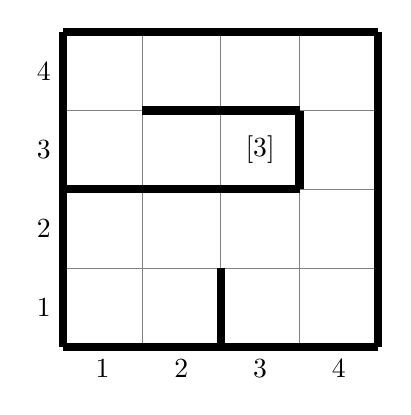
\begin{tikzpicture}
    \draw[step=1cm,gray,very thin] (0,0) grid (4,4);
    \foreach \x in {1, ..., 4}
      \draw (\x cm - .5cm, 1pt) -- (\x cm - .5cm, -1pt)
      node[anchor=north] {$\x$};
      \foreach \y in {1, ..., 4}
      \draw (1pt,\y cm - .5cm) -- (-1pt, \y cm - .5cm)
      node[anchor=east] {$\y$};
      
      % Goal
      \node (goal) at (2.5cm, 2.5cm) {\Coffeecup[3]};

      % Obstacles
      \draw[line width=3pt] (2cm, 0cm) -- (2cm, 1cm);
      \draw[line width=3pt] (0cm, 2cm) -- (3cm, 2cm);
      \draw[line width=3pt] (3cm, 2cm) -- (3cm, 3cm);
      \draw[line width=3pt] (3cm, 3cm) -- (1cm, 3cm);
      \draw[line width=3pt] (4cm, 4cm) -- (4cm, 3cm);

      % Border
      \draw[line width=3pt] (0cm, 0cm) -- (0cm, 4cm);
      \draw[line width=3pt] (0cm, 0cm) -- (4cm, 0cm);
      \draw[line width=3pt] (4cm, 4cm) -- (0cm, 4cm);
      \draw[line width=3pt] (4cm, 4cm) -- (4cm, 0cm);

      % Policy
      \node (1) at (.5cm, .5cm) {};  % (1,1)
      \node (1) at (1.5cm, .5cm) {}; % (2,1)
      \node (1) at (2.5cm, .5cm) {}; % (3,1)
      \node (1) at (3.5cm, .5cm) {}; % (4,1)
      
      \node (1) at (.5cm, 1.5cm) {};  % (1,2)
      \node (1) at (1.5cm, 1.5cm) {}; % (2,2)
      \node (1) at (2.5cm, 1.5cm) {}; % (3,2)
      \node (1) at (3.5cm, 1.5cm) {}; % (4,2)
      
      \node (1) at (.5cm, 2.5cm) {};  % (1,3)
      \node (1) at (1.5cm, 2.5cm) {}; % (2,3)
      %\node (1) at (2.5cm, 2.5cm) {}; % (3,3)
      \node (1) at (3.5cm, 2.5cm) {}; % (4,3)
      
      \node (1) at (.5cm, 3.5cm) {};  % (1,4)
      \node (1) at (1.5cm, 3.5cm) {}; % (2,4)
      \node (1) at (2.5cm, 3.5cm) {}; % (3,4)
      \node (1) at (3.5cm, 3.5cm) {}; % (4,4)
  \end{tikzpicture} &
  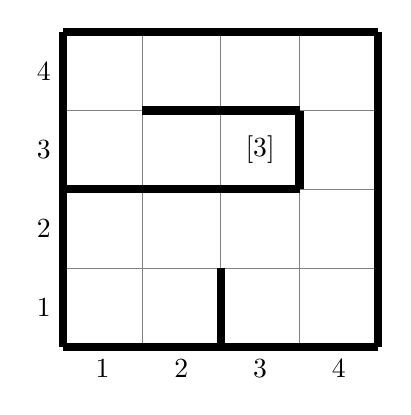
\begin{tikzpicture}
    \draw[step=1cm,gray,very thin] (0,0) grid (4,4);
    \foreach \x in {1, ..., 4}
      \draw (\x cm - .5cm, 1pt) -- (\x cm - .5cm, -1pt)
      node[anchor=north] {$\x$};
      \foreach \y in {1, ..., 4}
      \draw (1pt,\y cm - .5cm) -- (-1pt, \y cm - .5cm)
      node[anchor=east] {$\y$};
      
      % Goal
      \node (goal) at (2.5cm, 2.5cm) {\Coffeecup[3]};

      % Obstacles
      \draw[line width=3pt] (2cm, 0cm) -- (2cm, 1cm);
      \draw[line width=3pt] (0cm, 2cm) -- (3cm, 2cm);
      \draw[line width=3pt] (3cm, 2cm) -- (3cm, 3cm);
      \draw[line width=3pt] (3cm, 3cm) -- (1cm, 3cm);
      \draw[line width=3pt] (4cm, 4cm) -- (4cm, 3cm);

      % Border
      \draw[line width=3pt] (0cm, 0cm) -- (0cm, 4cm);
      \draw[line width=3pt] (0cm, 0cm) -- (4cm, 0cm);
      \draw[line width=3pt] (4cm, 4cm) -- (0cm, 4cm);
      \draw[line width=3pt] (4cm, 4cm) -- (4cm, 0cm);

      % Policy
      \node (1) at (.5cm, .5cm) {};  % (1,1)
      \node (1) at (1.5cm, .5cm) {}; % (2,1)
      \node (1) at (2.5cm, .5cm) {}; % (3,1)
      \node (1) at (3.5cm, .5cm) {}; % (4,1)
      
      \node (1) at (.5cm, 1.5cm) {};  % (1,2)
      \node (1) at (1.5cm, 1.5cm) {}; % (2,2)
      \node (1) at (2.5cm, 1.5cm) {}; % (3,2)
      \node (1) at (3.5cm, 1.5cm) {}; % (4,2)
      
      \node (1) at (.5cm, 2.5cm) {};  % (1,3)
      \node (1) at (1.5cm, 2.5cm) {}; % (2,3)
      %\node (1) at (2.5cm, 2.5cm) {}; % (3,3)
      \node (1) at (3.5cm, 2.5cm) {}; % (4,3)
      
      \node (1) at (.5cm, 3.5cm) {};  % (1,4)
      \node (1) at (1.5cm, 3.5cm) {}; % (2,4)
      \node (1) at (2.5cm, 3.5cm) {}; % (3,4)
      \node (1) at (3.5cm, 3.5cm) {}; % (4,4)
  \end{tikzpicture} \\
  \\
  East & West \\
  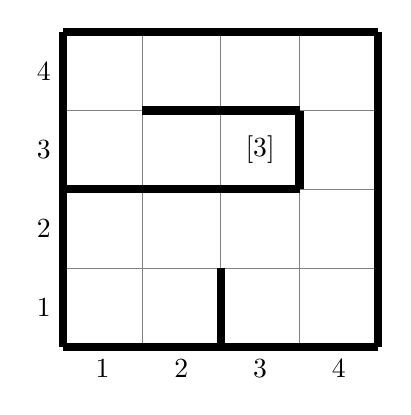
\begin{tikzpicture}
    \draw[step=1cm,gray,very thin] (0,0) grid (4,4);
    \foreach \x in {1, ..., 4}
      \draw (\x cm - .5cm, 1pt) -- (\x cm - .5cm, -1pt)
      node[anchor=north] {$\x$};
      \foreach \y in {1, ..., 4}
      \draw (1pt,\y cm - .5cm) -- (-1pt, \y cm - .5cm)
      node[anchor=east] {$\y$};
      
      % Goal
      \node (goal) at (2.5cm, 2.5cm) {\Coffeecup[3]};

      % Obstacles
      \draw[line width=3pt] (2cm, 0cm) -- (2cm, 1cm);
      \draw[line width=3pt] (0cm, 2cm) -- (3cm, 2cm);
      \draw[line width=3pt] (3cm, 2cm) -- (3cm, 3cm);
      \draw[line width=3pt] (3cm, 3cm) -- (1cm, 3cm);
      \draw[line width=3pt] (4cm, 4cm) -- (4cm, 3cm);

      % Border
      \draw[line width=3pt] (0cm, 0cm) -- (0cm, 4cm);
      \draw[line width=3pt] (0cm, 0cm) -- (4cm, 0cm);
      \draw[line width=3pt] (4cm, 4cm) -- (0cm, 4cm);
      \draw[line width=3pt] (4cm, 4cm) -- (4cm, 0cm);

      % Policy
      \node (1) at (.5cm, .5cm) {};  % (1,1)
      \node (1) at (1.5cm, .5cm) {}; % (2,1)
      \node (1) at (2.5cm, .5cm) {}; % (3,1)
      \node (1) at (3.5cm, .5cm) {}; % (4,1)
      
      \node (1) at (.5cm, 1.5cm) {};  % (1,2)
      \node (1) at (1.5cm, 1.5cm) {}; % (2,2)
      \node (1) at (2.5cm, 1.5cm) {}; % (3,2)
      \node (1) at (3.5cm, 1.5cm) {}; % (4,2)
      
      \node (1) at (.5cm, 2.5cm) {};  % (1,3)
      \node (1) at (1.5cm, 2.5cm) {}; % (2,3)
      %\node (1) at (2.5cm, 2.5cm) {}; % (3,3)
      \node (1) at (3.5cm, 2.5cm) {}; % (4,3)
      
      \node (1) at (.5cm, 3.5cm) {};  % (1,4)
      \node (1) at (1.5cm, 3.5cm) {}; % (2,4)
      \node (1) at (2.5cm, 3.5cm) {}; % (3,4)
      \node (1) at (3.5cm, 3.5cm) {}; % (4,4)
  \end{tikzpicture} &
  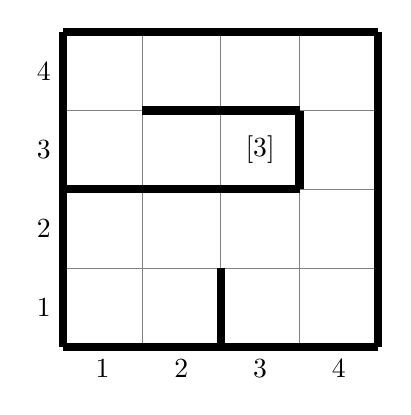
\begin{tikzpicture}
    \draw[step=1cm,gray,very thin] (0,0) grid (4,4);
    \foreach \x in {1, ..., 4}
      \draw (\x cm - .5cm, 1pt) -- (\x cm - .5cm, -1pt)
      node[anchor=north] {$\x$};
      \foreach \y in {1, ..., 4}
      \draw (1pt,\y cm - .5cm) -- (-1pt, \y cm - .5cm)
      node[anchor=east] {$\y$};
      
      % Goal
      \node (goal) at (2.5cm, 2.5cm) {\Coffeecup[3]};

      % Obstacles
      \draw[line width=3pt] (2cm, 0cm) -- (2cm, 1cm);
      \draw[line width=3pt] (0cm, 2cm) -- (3cm, 2cm);
      \draw[line width=3pt] (3cm, 2cm) -- (3cm, 3cm);
      \draw[line width=3pt] (3cm, 3cm) -- (1cm, 3cm);
      \draw[line width=3pt] (4cm, 4cm) -- (4cm, 3cm);

      % Border
      \draw[line width=3pt] (0cm, 0cm) -- (0cm, 4cm);
      \draw[line width=3pt] (0cm, 0cm) -- (4cm, 0cm);
      \draw[line width=3pt] (4cm, 4cm) -- (0cm, 4cm);
      \draw[line width=3pt] (4cm, 4cm) -- (4cm, 0cm);

      % Policy
      \node (1) at (.5cm, .5cm) {};  % (1,1)
      \node (1) at (1.5cm, .5cm) {}; % (2,1)
      \node (1) at (2.5cm, .5cm) {}; % (3,1)
      \node (1) at (3.5cm, .5cm) {}; % (4,1)
      
      \node (1) at (.5cm, 1.5cm) {};  % (1,2)
      \node (1) at (1.5cm, 1.5cm) {}; % (2,2)
      \node (1) at (2.5cm, 1.5cm) {}; % (3,2)
      \node (1) at (3.5cm, 1.5cm) {}; % (4,2)
      
      \node (1) at (.5cm, 2.5cm) {};  % (1,3)
      \node (1) at (1.5cm, 2.5cm) {}; % (2,3)
    %   \node (1) at (2.5cm, 2.5cm) {}; % (3,3)
      \node (1) at (3.5cm, 2.5cm) {}; % (4,3)
      
      \node (1) at (.5cm, 3.5cm) {};  % (1,4)
      \node (1) at (1.5cm, 3.5cm) {}; % (2,4)
      \node (1) at (2.5cm, 3.5cm) {}; % (3,4)
      \node (1) at (3.5cm, 3.5cm) {}; % (4,4)
  \end{tikzpicture}
  \end{tabular}\end{center}

\end{enumerate}

\subsubsection*{6. Q-Learning}

After many unsuccessful attempts at navigating to maze to find caffeine, the agent takes two major decisions.
\begin{itemize}
\item Tired of endlessly walking, the agent decides that from now on, it will explore this maze by skateboard. This mode of transportation is significantly faster than walking, so our agent will now always move \textbf{two blocks at a time}. For example, taking the action F in the state (1, 2, E) will result in the agent being in state (3, 2, E). If the agent is 1 block from the wall, it goes forward 1 and stops. 
\item Noticing the highly unoptimized layout of its environment, the agent decides to break three walls. The new environment is shown below (the red walls have been destroyed and can now be skateboarded over).
\end{itemize}


  \begin{center}\begin{tabular}{cc}
  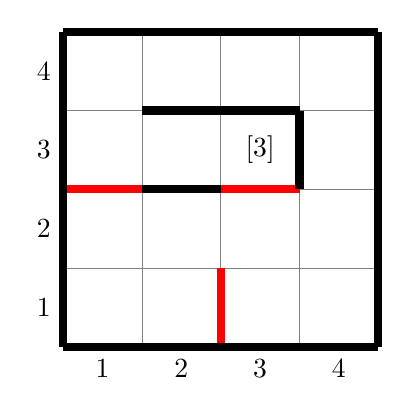
\begin{tikzpicture}
    \draw[step=1cm,gray,very thin] (0,0) grid (4,4);
    \foreach \x in {1, ..., 4}
      \draw (\x cm - .5cm, 1pt) -- (\x cm - .5cm, -1pt)
      node[anchor=north] {$\x$};
      \foreach \y in {1, ..., 4}
      \draw (1pt,\y cm - .5cm) -- (-1pt, \y cm - .5cm)
      node[anchor=east] {$\y$};
      
      % Goal
      \node (goal) at (2.5cm, 2.5cm) {\Coffeecup[3]};

      % Obstacles
      \draw[red, line width=3pt] (2cm, 0cm) -- (2cm, 1cm);
      \draw[red, line width=3pt] (0cm, 2cm) -- (1cm, 2cm);
      \draw[red, line width=3pt] (2cm, 2cm) -- (3cm, 2cm);
      \draw[line width=3pt] (1cm, 2cm) -- (2cm, 2cm);
      \draw[line width=3pt] (3cm, 2cm) -- (3cm, 3cm);
      \draw[line width=3pt] (3cm, 3cm) -- (1cm, 3cm);
      \draw[line width=3pt] (4cm, 4cm) -- (4cm, 3cm);

      % Border
      \draw[line width=3pt] (0cm, 0cm) -- (0cm, 4cm);
      \draw[line width=3pt] (0cm, 0cm) -- (4cm, 0cm);
      \draw[line width=3pt] (4cm, 4cm) -- (0cm, 4cm);
      \draw[line width=3pt] (4cm, 4cm) -- (4cm, 0cm);
  \end{tikzpicture} &
  \end{tabular}\end{center}

To best adapt to this new environment, you decide to use Q-Learning. Assume the learning rate $\alpha = 0.5$, the discount factor $\gamma=0.9$ and the following rewards: 
\begin{itemize}
\item The agent gets a reward of 10 for reaching the coffee cup
\item The agent gets a reward of -1 every time its movement goes through a broken wall, as the concrete debris damages the wheels of its skateboard
\end{itemize}

Because skateboarding is hard, \emph{transitions are no longer deterministic}. You \emph{do not know} the dynamics exactly, but instead have to look at sampled trajectories. Initialize the $Q$ function to zero again. Then for each of the episodes (trajectories) below, compute the updated $Q$ values. (Keep in mind that each computation below needs to take previous updates into account, and that all Q-values are initialized to 0.)


\begin{itemize}
    \item [] {[\textbf{1 point}]} i.) Beginning at the (1, 1, N) state, the agent skateboards action F and lands in (1, 3, N). It gets -1 reward for going over a broken wall. What is the updated $Q$ value at the starting state?\\ $Q(\texttt{(1, 1, N)}, \texttt{F})=$ \begin{tcolorbox}[fit,height=1cm, width=4cm, blank, borderline={1pt}{-2pt}]
    % solution 
    \end{tcolorbox}
    \item [] {[\textbf{1 point}]} ii.) Continuing from the (1, 3, N) state, the agent takes action R and is now in (1, 3, E). What is the update?\\ $Q(\texttt{(1, 3, N)}, \texttt{R})=$ \begin{tcolorbox}[fit,height=1cm, width=4cm, blank, borderline={1pt}{-2pt}]
    % solution 
    \end{tcolorbox}

    \clearpage
    
    \item [] {[\textbf{1 point}]} iii.) Beginning at the (1, 3, E) state, the agent takes action F and is now in (3, 3, E). It gets 10 reward for finding the coffee cup.\\ $Q(\texttt{(1, 3, E)}, \texttt{F})=$ \begin{tcolorbox}[fit,height=1cm, width=4cm, blank, borderline={1pt}{-2pt}]
    % solution 
    \end{tcolorbox}
    \item [] {[\textbf{1 point}]} iv.) If the agent started a new run at (1, 1, N) and was given the choice between actions F and R, what would the agent choose now? (Note that the agent is not actually choosing this action and is not updating the $Q$ function.) $a=$ \begin{tcolorbox}[fit,height=1cm, width=4cm, blank, borderline={1pt}{-2pt}]
    % solution 

    \end{tcolorbox}
    \item [] {[\textbf{1 point}]} v.) Now the agent starts a new episode at the (1, 3, N) state. The agent takes action R and is now in (1, 3, E). \\ $Q(\texttt{(1, 3, N)}, \texttt{R})=$ \begin{tcolorbox}[fit,height=1cm, width=4cm, blank, borderline={1pt}{-2pt}]
    % solution 
    \end{tcolorbox}
    \item [] {[\textbf{1 point}]} vi.) Npw the agent starts a new episode at the (1, 1, N) state. The agent skateboards action F and lands in (1, 3, N). It gets -1 reward for going over a broken wall.\\ $Q(\texttt{(1, 1, N)}, \texttt{F})=$ \begin{tcolorbox}[fit,height=1cm, width=4cm, blank, borderline={1pt}{-2pt}]
    % solution 
    \end{tcolorbox}
    \item [] {[\textbf{1 point}]} vii.) Now if the agent started a new run at (1, 1, N) and was given the choice between actions F and R, what would the agent choose? (Again, do not actually update the $Q$ function.) $a=$ \begin{tcolorbox}[fit,height=1cm, width=4cm, blank, borderline={1pt}{-2pt}]
    % solution 
    \end{tcolorbox}
    \item [] {[\textbf{2 points}]} viii.) If transitions \textit{were} deterministic, the optimal sequence of actions from (1, 1, N) would be F, R, F. However, we no longer have that guarantee. Assuming all other transitions in all other states are deterministic, give a simple example of transition probabilities for the actions at (1, 1, N) for which the learned optimal move at (1, 1, N) is not F.

    \begin{tcolorbox}[fit,height=4cm, width=17cm, blank, borderline={1pt}{-2pt},nobeforeafter]
    %solution

    \end{tcolorbox}
    
    
\end{itemize}
